\section{Statistical Analysis of Mock Dataset}

There are $5$ plain text files given, called $v_1$, $v_2$, $v_3$, $v_4$ and $v_5$. ($v_1$ is
short for variable $1$, \etc{}) Each text file contains $1600000$ lines, which correspond to
measurements of the given variable from a simulation. There are autocorrelations
(correlations in time or measurement number) for each variable. There are also correlations
between variables. In this problem, you need to analyze this data, using the methods
discussed in class, to find average values, standard deviations of means, autocorrelations,
etc.

We will use $M$ to represent the total number of values, i.e. $M = 1600000$. $M$ is large
enough so that it represents an effectively ``infinite'' sample size. Thus, the true data
mean can be well approximated by averaging over all $M$ values. Averages, standard
deviations, \etc. determined from the ``infinite'' sample will be denoted with a hat, i.e.
$\barhat{v}_1$, \etc.

We will use $N$ to represent the number of measurements in a sample of the data. $N$
corresponds to the amount of data you might actually collect in a simulation.

\Question{} Determine the true means, $\barhat{v}_a$ for $v_1$, $v_2$, $\ldots$, $v_5$ from
all $M$ values.

\Answer{}
First, we need to read the data from each file. This is pretty simple since all $5$ files
are plain text files. The method is shown in function \code{readdata} in
Snippet~\ref{lst:readdata}.

\begin{algorithm}[H]
    \caption{Function \code{readdata} reads the data from each file.}
    \label{lst:readdata}
    \begin{juliacode}
        function readdata(filename)
            open(filename, "r") do io
                return map(eachline(io)) do line
                    parse(Float64, strip(line))
                end
            end
        end
    \end{juliacode}
\end{algorithm}

The definition of the true mean is
\begin{equation}
    \barhat{v} = \bigl \langle \bar{v} \bigr \rangle = \frac{ 1 }{ M } \sum_{i=1}^{M} v_i.
\end{equation}

Therefore, the true means, $\barhat{v}_a$ for $v_1$, $v_2$, $\ldots$, $v_5$ from
all $M$ values are shown in Table~\ref{tab:truemean}.

\begin{table}[H]
    \centering
    \caption{The true means $\barhat{v}_a$ from all $M$ values.}
    \label{tab:truemean}
    \begin{tabular}{@{}ccccc@{}}
        \toprule
        $\barhat{v}_1$ & $\barhat{v}_2$ & $\barhat{v}_3$ & $\barhat{v}_4$ & $\barhat{v}_5$ \\
        \midrule
        1.76084        & 2.88634        & 4.01185        & 5.13712        & 6.26238        \\
        \bottomrule
    \end{tabular}
\end{table}

\Question{} Consider two values for our sample size: $N = 1000$ and $N = 10000$. There are
$M/N$ samples of this size in our $M$ values. Histogram the sample means for these values of
$N$ and determine the true standard deviation of the means $\hat{\sigma}_{\barhat{v}_a,N}$.
You can determine $\hat{\sigma}_{\barhat{v}_a,N}$ by assuming each of the $M/N$ samples is
independent. This is reasonable, provided the autocorrelations in the data are smaller than
the values of $N$ you use. Do your two values for $\hat{\sigma}_{\barhat{v}_a,N}$ show the
correct behavior with $N$?

\Answer{}

There are $1600$ and $160$ samples for $N = 1000$ and $N = 10000$, resepectively.
We calculate their means and plot them in histograms, as shown in
Figures~\ref{fig:hist_mean:a} and~\ref{fig:hist_mean:b}.
We can see that the distribution of the mean values changes in Figure~\ref{fig:hist_mean:b}
since more values are averaged.

\begin{figure}[h]
    \centering
    \begin{minipage}[t]{0.8\linewidth}
        \centering
        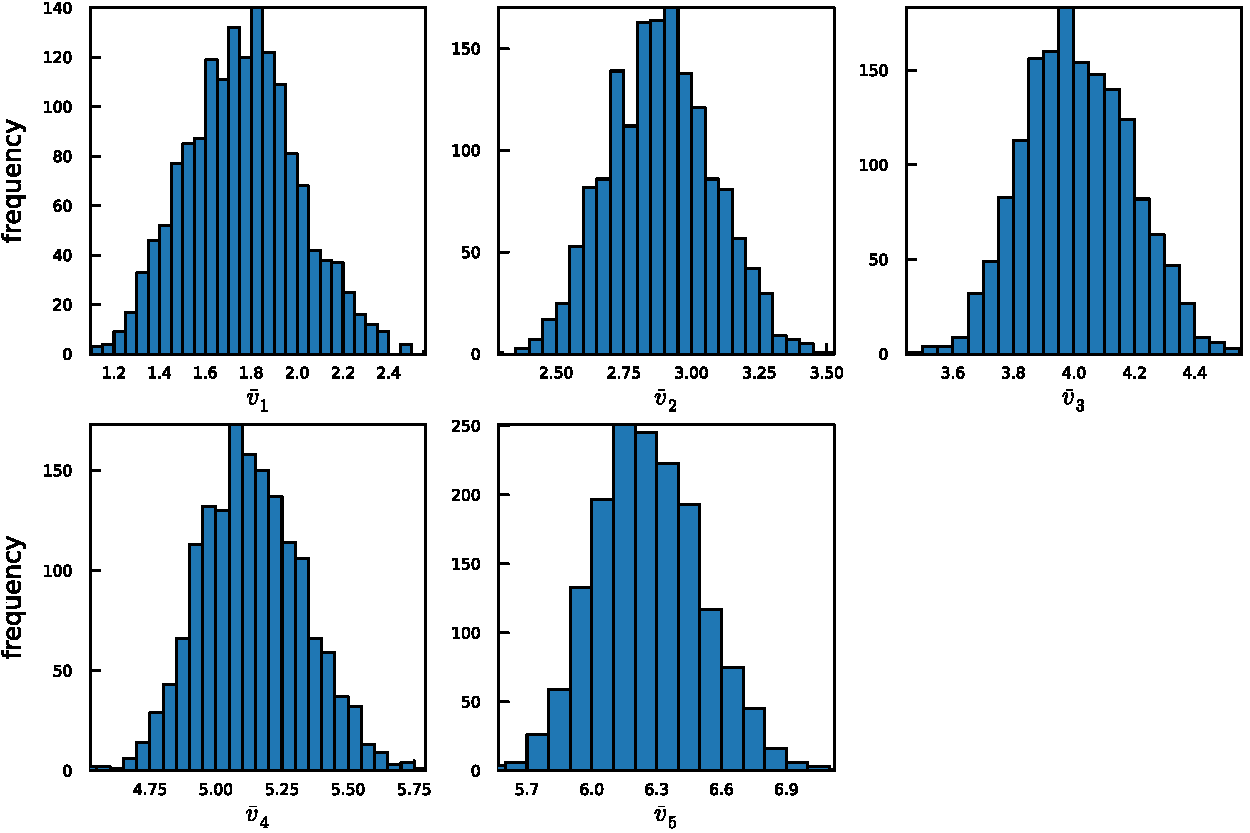
\includegraphics[width=\linewidth]{sample means N=1000}
        \subcaption{Histogram of the sample means for $N = 1000$.}
        \label{fig:hist_mean:a}
    \end{minipage}
    \hfill
    \begin{minipage}[t]{0.8\linewidth}
        \centering
        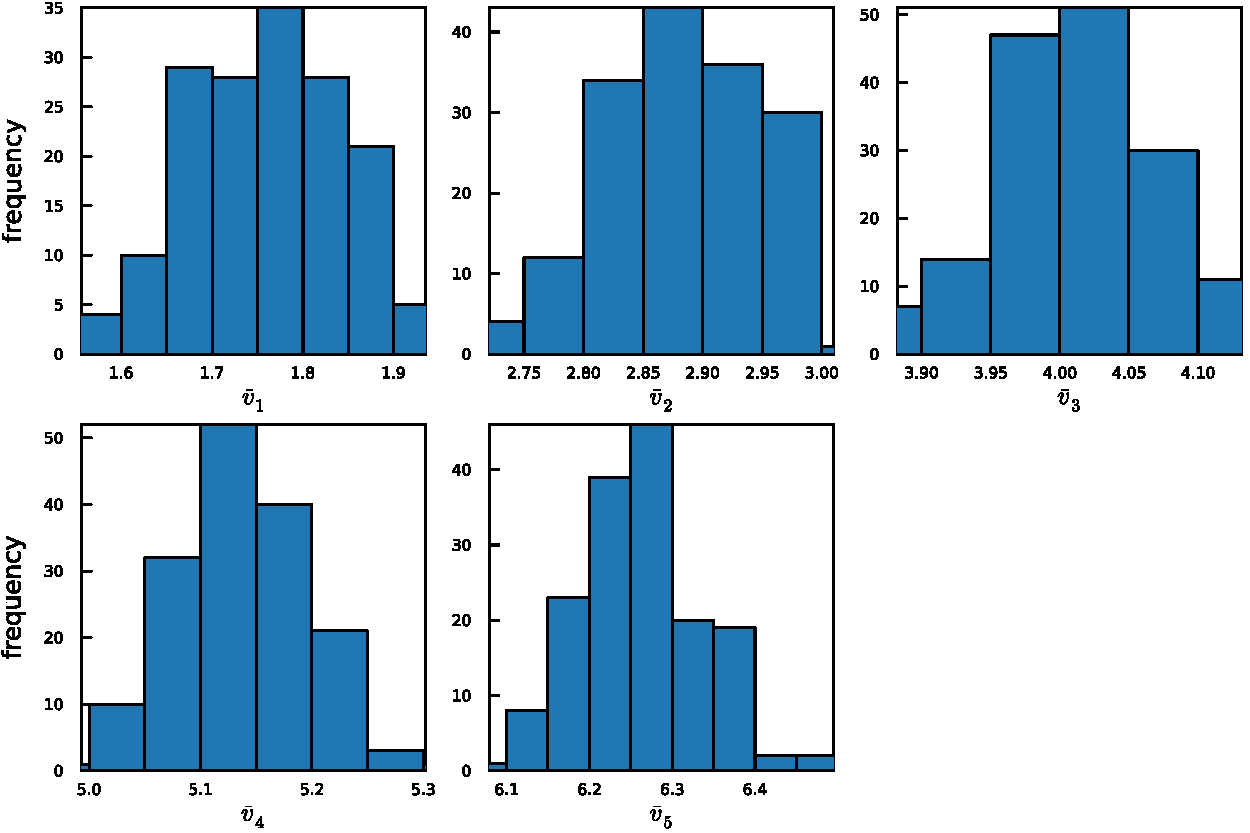
\includegraphics[width=\linewidth]{sample means N=10000}
        \subcaption{Histogram of the sample means for $N = 10000$.}
        \label{fig:hist_mean:b}
    \end{minipage}
    \label{fig:hist_mean}
    \caption{Take $N = 1000$ and $N = 10000$ as each sample size
        for $v_1$, $v_2$, $\ldots$, $v_5$ from all $M$ values
        and histogram their mean values.}
\end{figure}

The true variance is defined as

\begin{equation}
    \hat{\mathbb{V}}(v) = \frac{ 1 }{ M/N - 1 }
    \sum_{\eta=1}^{M/N} (\bar{v}_\eta - \barhat{v})^2.
\end{equation}
